
\section{Introduction}
Recently, Proxy Mobile IPv6 (PMIPv6) \cite{PMIPv6} has been standardized by the IETF, and widely adopted in 3GPP and WiMAX architecture. Taking advantage of the network-based mobility management, PMIPv6 enables IP mobility for moving hosts without their involvement. PMIPv6 brings several benefits compared to the host-based mobility management (e.g., MIPv6 \cite{MIPv6}) (see Chapter \ref{ch:reference_technologies}). However, PMIPv6 fails to support the inter-domain mobility. That means, even when an MN moves to another PMIPv6 domain, session continuity cannot be maintained.

In order to support the inter-domain mobility, several solutions have been proposed e.g., integration of MIPv6 and PMIPv6 (H-PMIP) \cite{rfc6612}; and I-PMIP \cite{i-pmip}. Yet, they have limitations such as sub-optimal routing, signaling overhead and handover latency. Especially, due to the lack of granularity on the mobility management service, the mobility service is always provided even for the sessions that do not require mobility management support e.g., the sessions launch and complete while the mobile node connected to the same domain. 

In this chapter, we propose inter-domain mobility solutions for PMIPv6 (called D-PMIP) based on the DMM concept. Following the DMM requirement (REQ4) in terms of reusing/extending the existing IETF IP mobility protocols (i.e., MIPv6 and PMIPv6), the proposed solutions apply the DMM concept into the existing PMIPv6 networks to support inter-domain mobility. The solutions may be fully or partially distributed. Thus, they allow data packets to be routed via a near-optimal way by bringing the mobility anchors closer to the MN while the control management can be placed anywhere in the network. The numerical results show that the partially distributed solution (DP-PMIP) gives better performance than the existing inter-domain handover solutions e.g., MIPv6, H-PMIP and I-PMIP in terms of handover latency, signaling cost and tunnel usage. 

The rest of this chapter is organized as follows. Section \ref{ch9:related_work} describes related work on the inter-domain mobility support. In section \ref{ch9:solution_description}, the two different proposals are presented with respect to its architecture and operations. We also present a basic support for the multicast listener mobility in the proposed solution. Section \ref{ch9:performance_analysis} provides performance analysis in terms of signaling cost, handover latency and tunnel usage. Section \ref{ch9:numerical_result} shows the numerical results taking into account the impact of different factors. Eventually, Section \ref{ch9:conclusion} concludes this chapter.  

\section{Inter-domain Mobility Support} \label{ch9:related_work}
Several solutions have been proposed for inter-domain mobility support for PMIPv6. The common idea is using a global mobility anchor to keep the MN reachable when it moves to a visited PMIPv6 domain. In \cite{rfc6612}, the authors introduce a scenario in which PMIPv6 is used as an intra-domain mobility management whereas MIPv6 as a global mobility management (named H-PMIP). As a result, the complexity of the hosts is increasing since they have to support both the network-based and the client-based protocol stacks. Another scenario is also considered, where PMIPv6 and MIPv6 are co-located at LMA/HA. Yet, there exist some problems due to the natural difference between the two protocols \cite{rfc6612}.  

In \cite{i-pmip}, an extension to PMIPv6 (called I-PMIP) is proposed for the inter-domain mobility support by reusing the local mobility anchor as a global anchor point when the MN is away from home. Then the traffic is forwarded from/to the anchor, which is called Session Mobility Anchor (SMA), to/from the current serving Local Mobility Anchor (S-LMA) where the MN is currently attached. Thus, two scenarios are suggested to find the corresponding SMA:
\begin{itemize}
\item Direct location: A common database is introduced to store information about the established MN-SMA bindings from all domains. 
\item Indirect location: This scenario is based on the fact that the SMA is a topological anchor point of the MN. So, after inferring the MN's IPv6 address, the S-LMA sends a PBU to this address. This PBU will obviously reach the SMA. However, this approach requires each SMA to analyze all of its incoming traffic to recognize the corresponding PBU. As a result, the complexity of the LMA is increasing, particularly when a lot of traffic passes the LMA.     
\end{itemize} 

One critical problem of this solution is that the mobility service is provided on a per user basis. Thus, the mobility service is always provided even for the sessions that do not require a mobility support (e.g., when the MN remains attached to the same domain during the lifetime of the sessions). Also, when the MN starts a new session at a new domain, it still has to use the SMA as the anchor point, which may cause the sub-optimal routing and tunneling overhead problems.

Another proposal \cite{draft-ma} is based on the idea that the home address (HoA) and Care-of-Address (CoA) are not only used for the MN, but also for the specific session. Every PMIPv6 entity maintains two Binding Cache Entries (BCE) for each registered MN. One is Inner-domain BCE as normal BCE in the PMIPv6 domain, and the other is Inter-domain BCE which maintains the binding between HoA and CoA of the Corresponding Node (CN). When an MN moves to another PMIPv6 domain, the S-LMA needs to communicate with the previous one to get the HoA of CN. It also interacts with the CN's home LMA to update the current location of the MN. The same process is executed when CN changes its PMIPv6 domain. Though the traffic is routed via a near-optimal way (directly from the CN to the current location of the MN), this solution becomes too complex especially when the MN communicates with many CNs at the same time. Moreover, this proposal can be applied only in the case where both the MN and the CN are attached to PMIPv6 domains. 

\section{Description of the Solution} \label{ch9:solution_description}
Based on the DMM concept, we introduce an inter-domain mobility support, called D-PMIP. Thus, this proposal brings some benefits: (i) the mobility anchors are placed very close towards the MN; and (ii) the mobility service is only provided for the sessions that really require the service continuity.  

Once the MN enters its PMIPv6 domain, it gets a set of prefixes. For simplicity, it is assumed that only one prefix will be allocated for each MN. Based on the prefix allocated, the MN configures its IPv6 address. The MN then can use this address to initiate and maintain the sessions in a standard way while it remains attached to this domain. When the MN changes its domain, it gets another prefix and configures its address based on this prefix. This address can be used to set up the new sessions. Until the previous sessions are not closed, the old address should be kept. Thus, a tunnel is built between the anchor LMA (A-LMA) and the current one to redirect packets between two LMAs using the old prefix. 

To enable the inter-domain mobility support, the BCE in the LMA is needed to extend with a field, called I-LMA which contains a list of the MN's prefixes and the previous/current LMA's address. Based on the DMM concept, two possible solutions for inter-domain mobility support are considered, namely the partially (DP-PMIP) and fully distributed (DF-PMIP) solution. The former solution relies on a common database for control plane, while in the latter one the mobility function is distributed in both data and control plane. 
\subsection{Partially Distributed Solution (DP-PMIP)}

Similar to I-PMIP, this solution relies on the existing of a central entity called Inter-domain Central Mobility Database (ICMD) which stores information of mobility sessions of all PMIPv6 domains. This common database can be established by service level agreements between the operators of PMIP domains. Unlike I-PMIP, the MN's prefix is used to distinguish between ICMD entries. In addition, the ICMD can play the role of the LMA and the MAG to handle the PBU/ PBA messages. 
\subsubsection{Initial Registration}
\begin{figure}[h!]
\centering
\includegraphics[width=0.65\textwidth]{./Part3/Chapter7/figures/c9_registration.eps}
\caption[Initial registration signaling in the partially distributed approach.]{Initial registration signaling in the partially distributed approach (DP-PMIP).}
\label{fig:c9_registration}
\end{figure}

When an MN is attached to a PMIPv6 domain, the standard PMIPv6 operations are executed. The LMA (LMA1) then sends a PBU to the ICMD. This PBU includes the Mobile Node Identifier and Home Network Prefix (HNP) option which are set to the MN's identifier (MN-ID) and the MN's prefix (Pref1), respectively. Since the session is new, the ICMD creates an entry which consists of the MN-ID, the Pref1 and the address of LMA1 in its BCE. The signaling process and the BCE of the ICMD are described in Fig.~\ref{fig:c9_registration}.
\subsubsection{Inter-domain Operations}
\begin{figure}[h!]
\centering
\includegraphics[width=0.95\textwidth]{./Part3/Chapter7/figures/c9_handover.eps}
\caption[Handover signaling in the partially distributed approach.]{Handover signaling in the partially distributed approach (DP-PMIP).}
\label{fig:c9_handover}
\end{figure}

The signaling procedure of DP-PMIP in case of handover is illustrated in Fig.~\ref{fig:c9_handover}. When the MN moves to another domain, the current LMA (LMA2 or S-LMA) allocates another prefix (Pref2) to the MN. Then, the S-LMA sends a PBU to the ICMD for the new prefix registration. Upon receiving the PBU and searching the BCE table, the ICMD updates the current location to the existing entries for the MN. It also creates a new entry corresponding to the MN-ID and the new prefix. The ICMD then sends a PBU including the S-LMA's address to the A-LMA (LMA1) to update the current location of the MN. After receiving the PBU, the A-LMA sets up its endpoint for bi-directional tunnel to the S-LMA, updates its BCE and routing for Pref1. In parallel, the ICMD indicates the address of A-LMA to S-LMA (by means of PBA message), which performs the same process as that of A-LMA. Afterwards, a bi-directional tunnel is established between the S-LMA and A-LMA to carry the traffic from/to MN using Pref1.

As a global anchor point of Pref1, the A-LMA, after receiving the packets destined to this prefix, forwards them through the bi-directional tunnel to the corresponding S-LMA. The packets then reach the MN at the current PMIPv6 domain. 

When the MN transmits packets using Pref1 as source, the S-LMA, after receiving the packets, firstly checks their source address in the BCE. The S-LMA then forwards them through the tunnel to the corresponding A-LMA which routes them towards the destination. On the contrary, the packets using Pref2 as source are routed as a regular PMIPv6 routing.

\subsection{Fully Distributed Solution (DF-PMIP)}
\begin{figure}[h!]
\centering
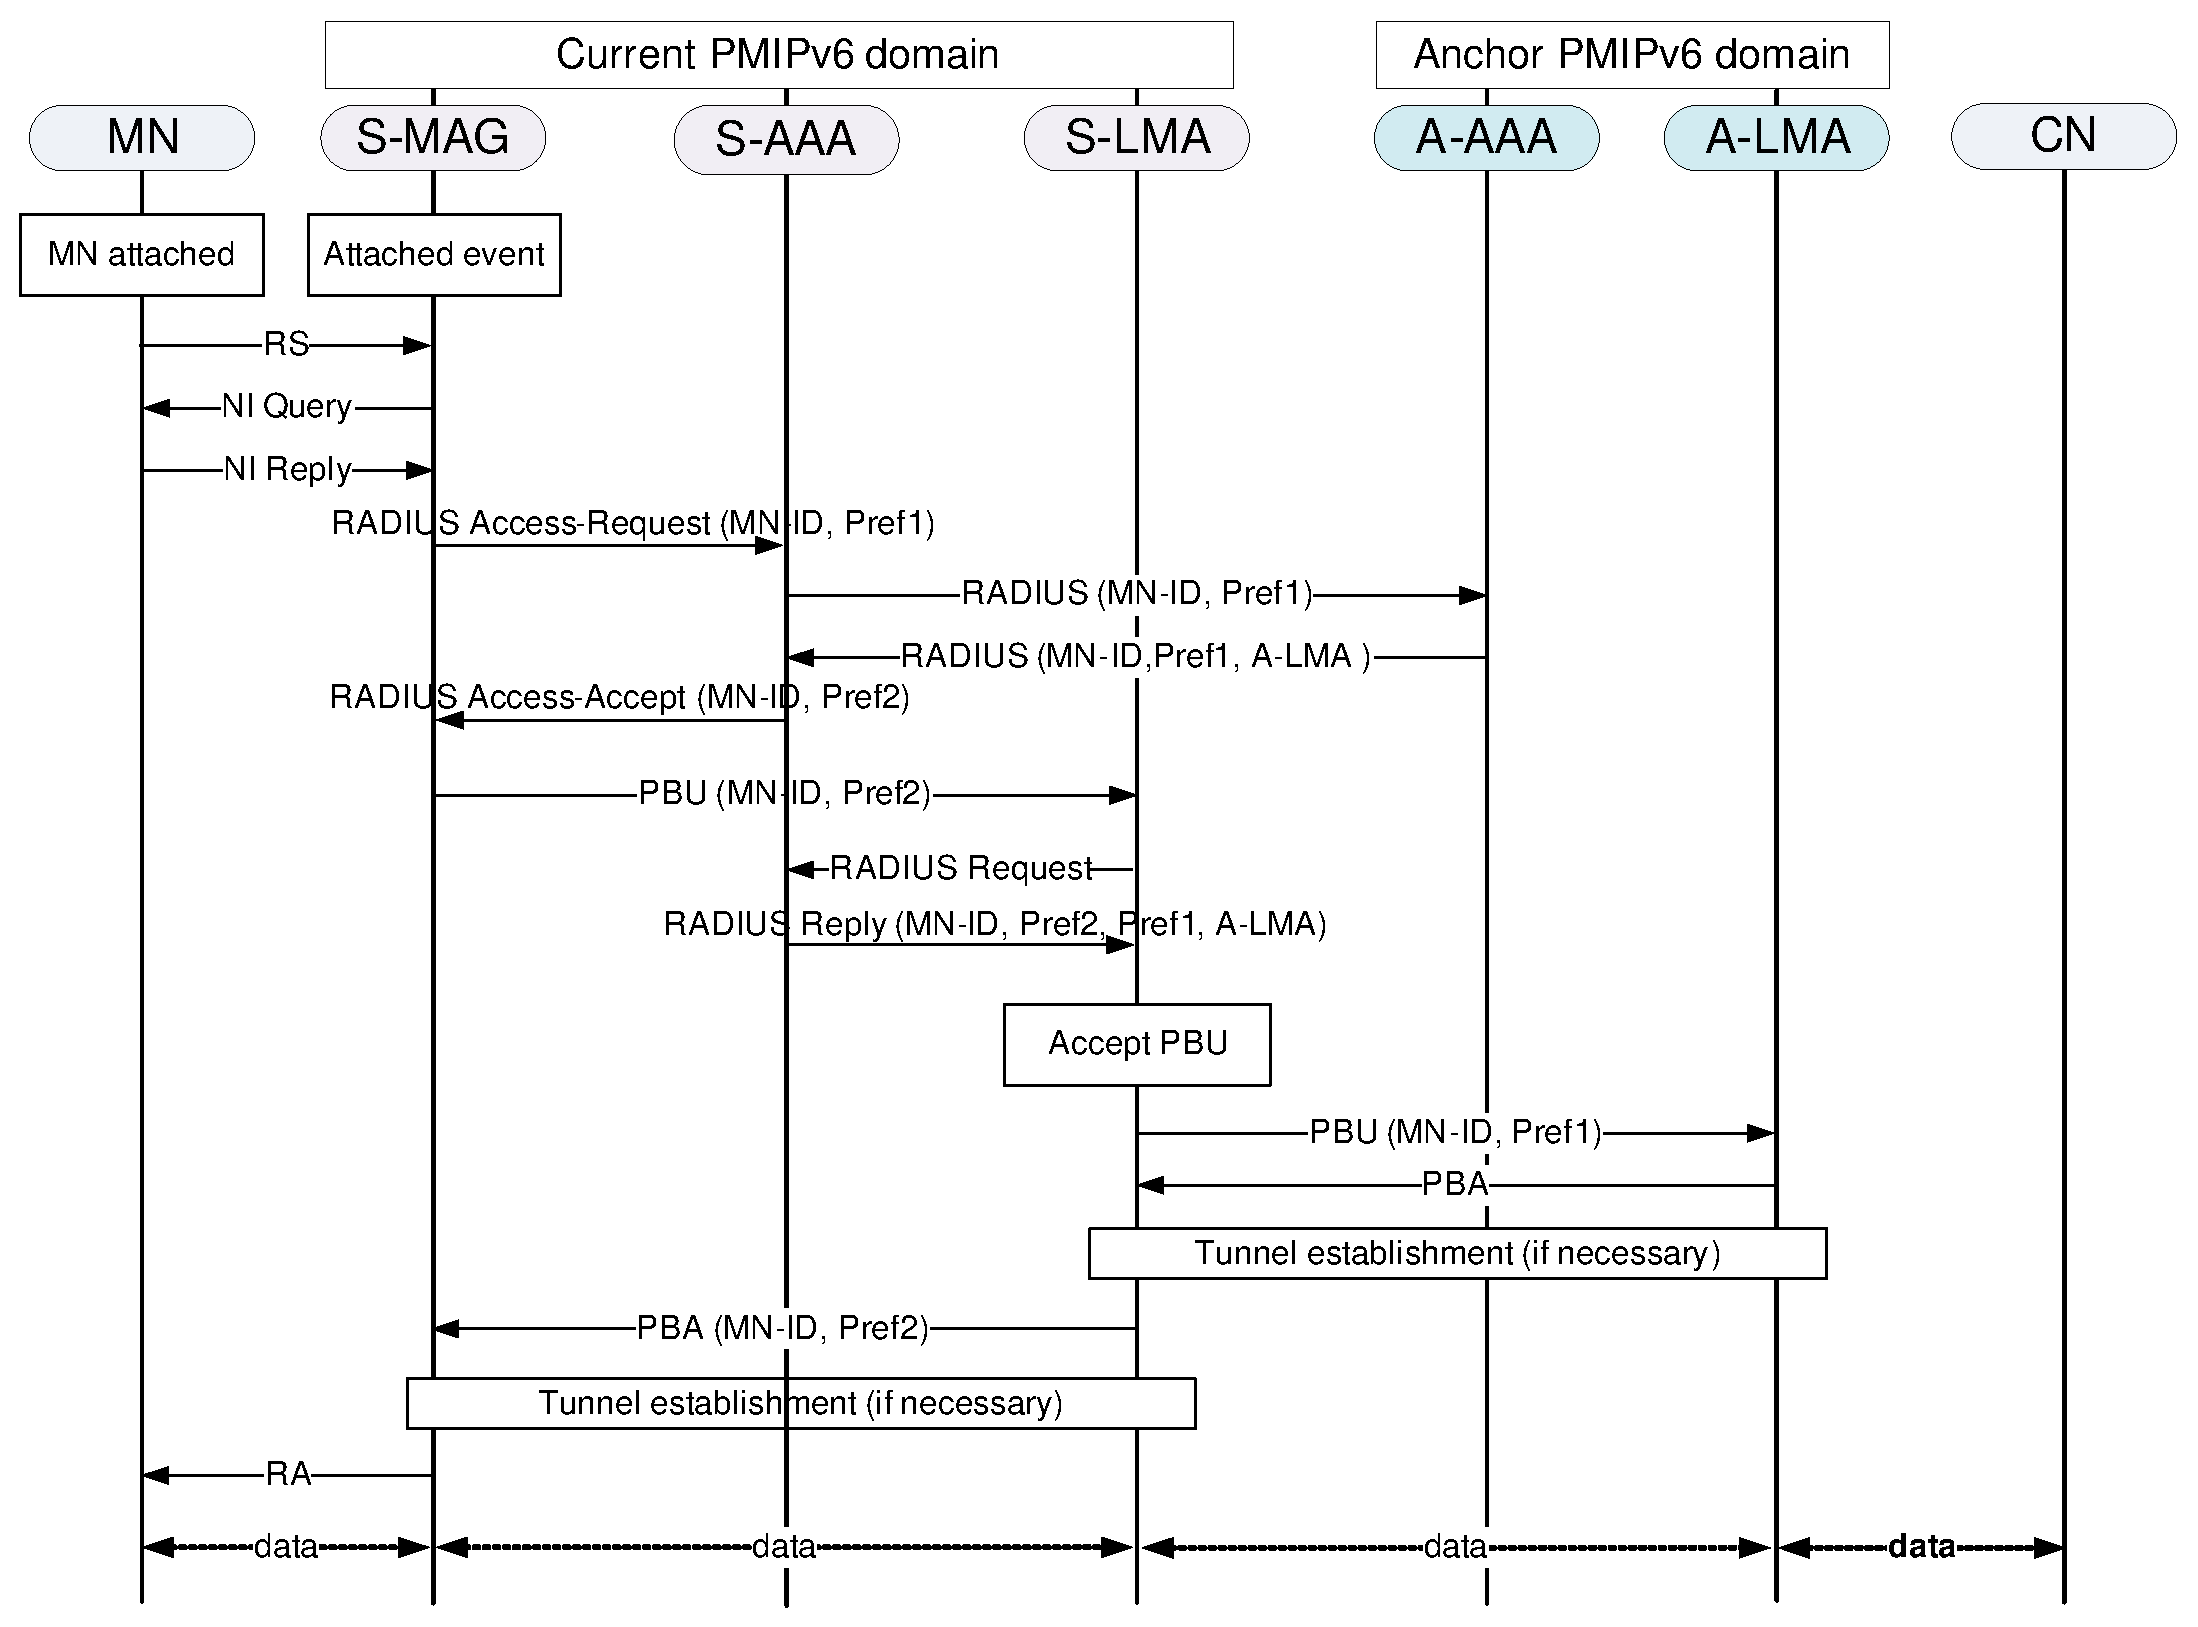
\includegraphics[width=0.95\textwidth]{./Part3/Chapter7/figures/c9_fully_distributed.eps}
\caption[Signaling for the fully distributed approach.]{Fully distributed approach (DF-PMIP).}
\label{fig:c9_fully_distributed}
\end{figure}

In this solution, the central database for inter-domain is removed from the architecture. Thus the complexity of the handover procedures is increased as a result of the trade-off between the elimination of the central database and the signaling cost. Since the S-LMA does not have knowledge of the LMAs in the other PMIPv6 domain, finding the A-LMA's address of the MN's prefix becomes a key challenge. There are several methods to solve this issue:
\begin{itemize}
\item using a Layer 2 handover infrastructure e.g., IEEE 802.21 \cite{IEEE802.21};
\item using a distributed LMA-discovery mechanism \cite{lma_discovery};
\item relying on a distributed infrastructure that allows the communication between the domains. 
\end{itemize}

In this chapter, we introduce an example to illustrate how this approach works by using a distributed Authentication, Authorization, and Accounting (AAA) infrastructure \cite{aaa2} and Remote Authentication Dial In User Service (RADIUS) protocol for PMIPv6 \cite{radius}. The protocol operations can be briefly explained as follows (see Fig.~\ref{fig:c9_fully_distributed}). 

After detecting the presence of a new MN, the current serving MAG (S-MAG) obtains the information of the MN (MN's IPv6 address) by exchanging Node Information (NI) Query/NI Reply messages \cite{rfc4620}. If the MN's IPv6 address is not available, then the normal process is executed. Vice versa, the S-MAG, after extracting the prefix from MN's address, sends a RADIUS Access-Request message with PMIPv6-Home-HN-Prefix (Pref1) and Mobile-Node-Identifier (MN-ID) options, to the AAA server (S-AAA) to retrieve the MN's policy profile. If this prefix belongs to its domain, the S-AAA then continues with its regular operations. Otherwise, acting as a RADIUS client, the S-AAA sends a RADIUS message (including MN-ID and Pref1) to the AAA in the anchor domain (A-AAA), to get A-LMA's address. Upon the reception of the RADIUS reply message from A-AAA, the S-AAA sends an Access-Accept message which includes the prefix allocated to this MN (Pref2) to S-MAG. Afterwards, the standard PMIP operations related to Pref2 are executed (e.g., location update and MN's address configuration). The S-LMA also obtains the A-LMA address from the S-AAA server. Then, the PBU/PBA messages are exchanged between the S-LMA and A-LMA to update their BCEs and routing related to Pref1. 

\subsection{Local Routing Considerations}
After the receipt of the up-link packets from MN using Pref1 as source, the S-LMA will decide to forward them to the destination depending on the following cases: (i) if the CN is currently attached to its domain, the S-LMA simply forwards the packet to the corresponding MAG; (ii) if the CN's address belongs to its domain but the CN is currently attached to another one, the S-LMA will forward the packets to the LMA that the CN is currently attached to; and iii) Otherwise, the packets will be routed following the normal internet routing. 
\subsection{Multicast Considerations}
All proposals for the inter-domain mobility support do not take multicast into account. In general, when a listener moves to a new domain, the on-going multicast flows will be interrupted. Additionally, the MN then has to re-join these flows in the new domain. Thus, the main objectives are: i) keeping the MN unaware of mobility from multicast application point of view; and ii) reducing the potential service disruption. 
In our proposed solution, multicast support can be enabled by using the multicast context transfer function and extending the PBU/PBA message to convey the multicast subscription information of the MN, as described in Fig\ref{fig:c9_multicast_signaling}. As stated in the previous section, the multicast context transfer function is developed as an independent module, which allows it to be easily integrated in any solution. 
\begin{figure}[h!]
\centering
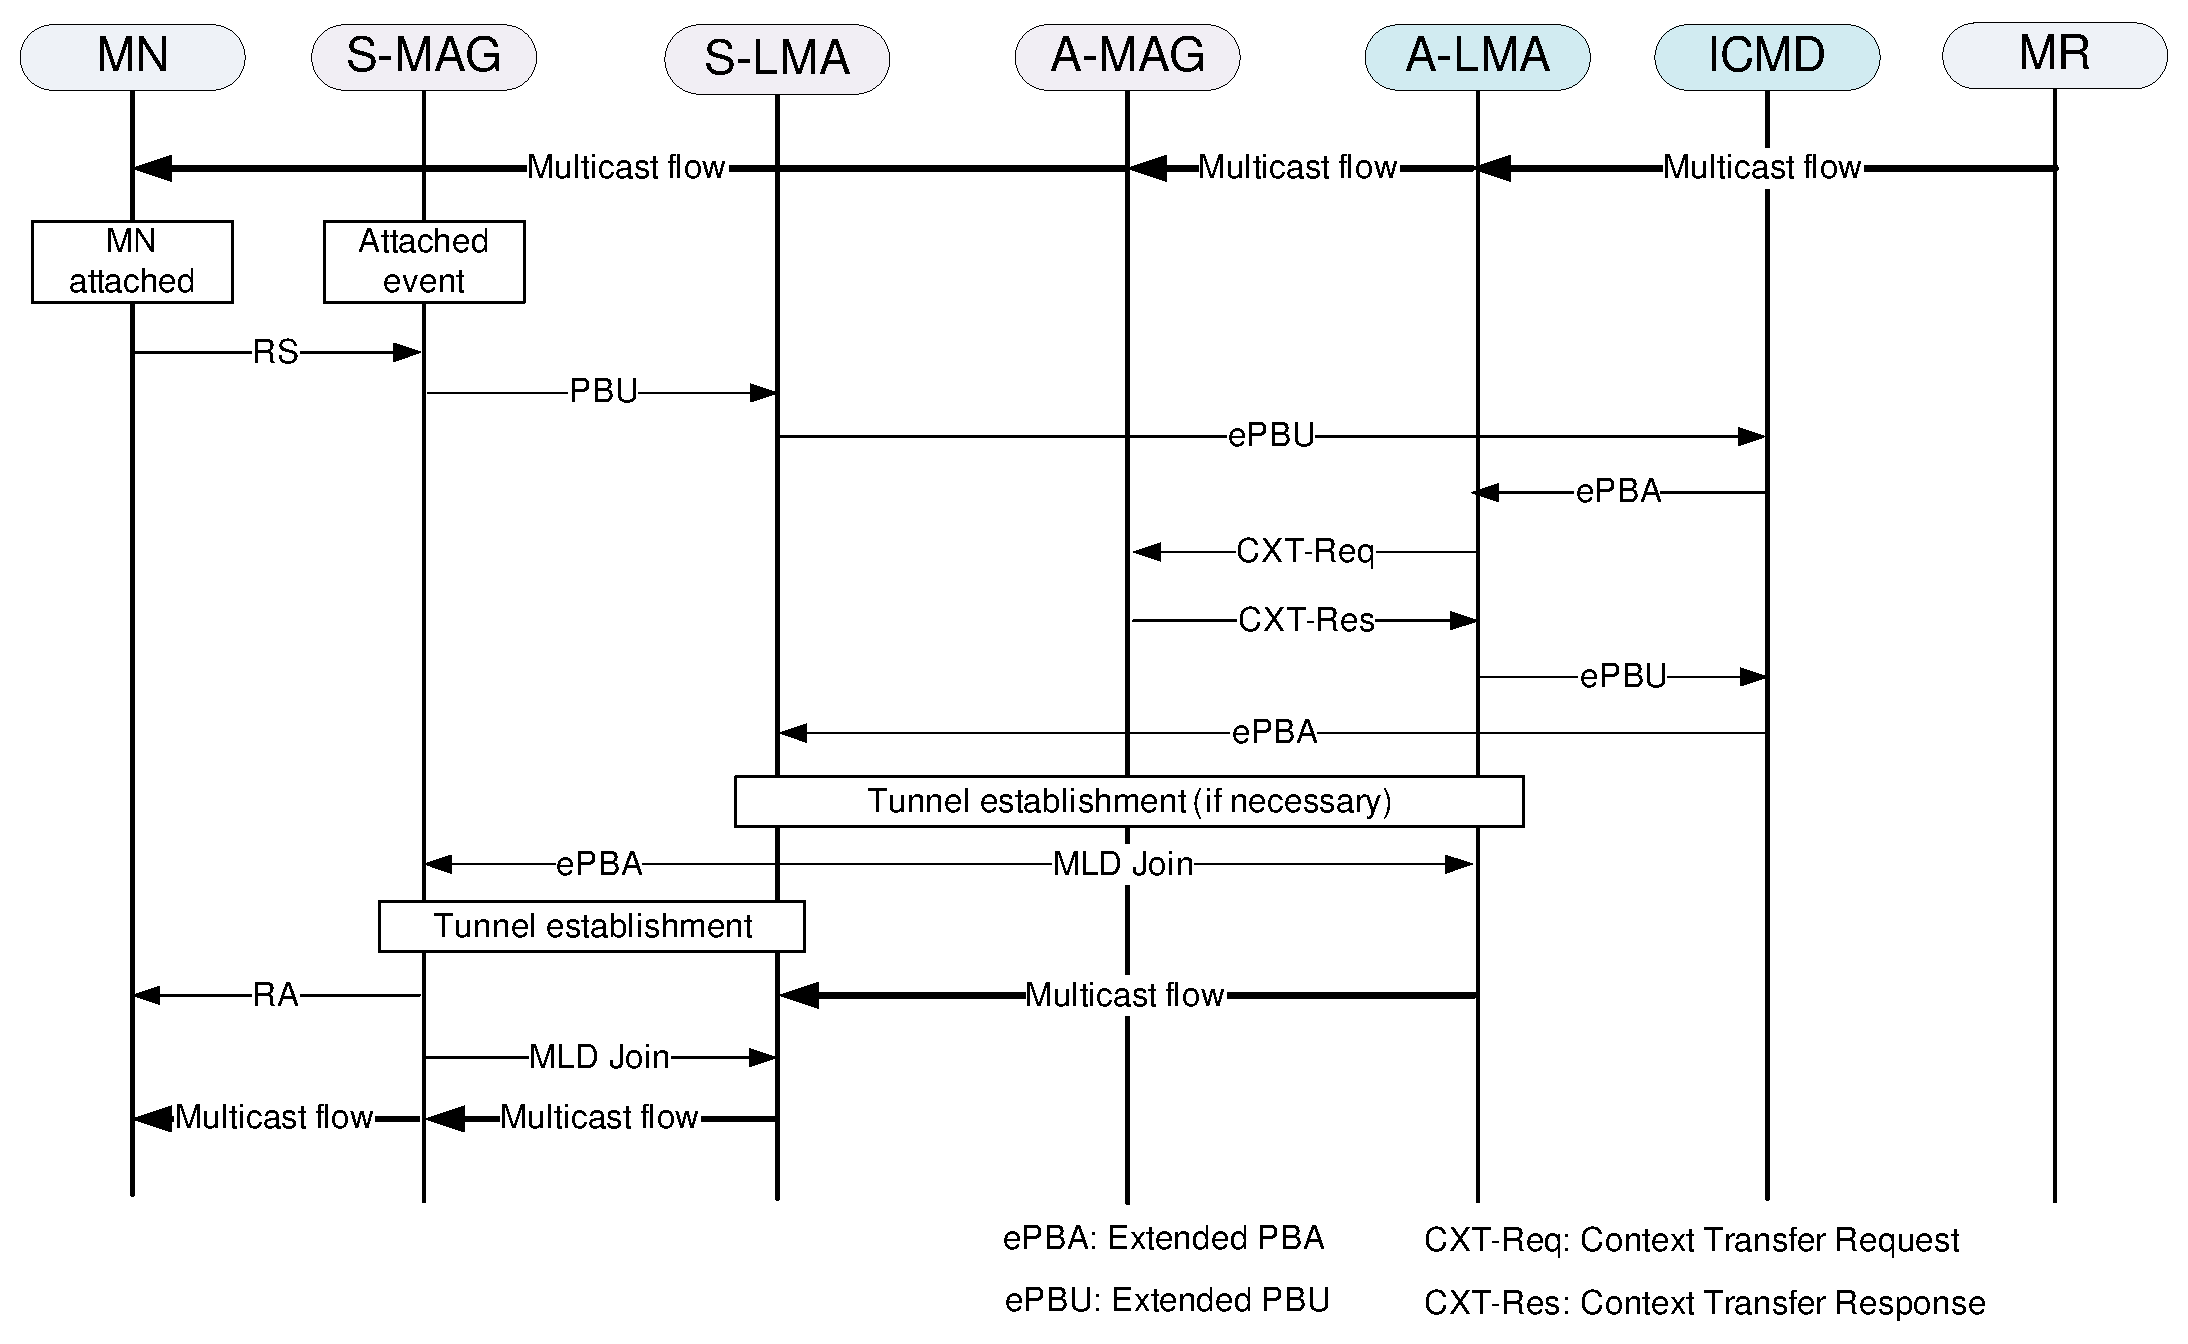
\includegraphics[width=0.85\textwidth]{./Part3/Chapter7/figures/c9_multicast_signaling.eps}
\caption[Multicast mobility support in the inter-domain mobility solution.]{Multicast mobility support in DP-PMIP.}
\label{fig:c9_multicast_signaling}
\end{figure}
The multicast-related signaling process is briefly described as follows. As stated in the previous section, upon the reception of PBU from the S-LMA, the ICMD sends a PBA to the A-LMA to update the current location of the MN. This PBA is extended to request the multicast subscription information of the MN. The A-LMA based on the context transfer function obtains the MN's subscription information from the A-MAG, and then sends it to the ICMD. The ICMD replies to the S-LMA by sending a PBA message including the MN's subscription information. The S-LMA, after establishing a tunnel with the A-LMA, sends an MLD Report to join the ongoing multicast flows of the MN via the A-LMA. The S-LMA also includes the subscription information in the PBA message to send to the S-MAG. The S-MAG, after adding the MN to a downstream interface of its MLD proxy, sends an MLD Report to the S-LMA to join these flows. Afterwards, the multicast packets are routed to the MN via the A-LMA, S-LMA and S-MAG.
\section{Performance Analysis}\label{ch9:performance_analysis}
In this section we analyze the performance of the proposed solutions in terms of signaling cost, handover latency and tunnel usage. We compare our solutions with the other ones for the inter-domain handover e.g., MIPv6, H-PMIP and I-PMIP. 
\subsection{Reference Model}
\begin{figure}[h!]
\centering
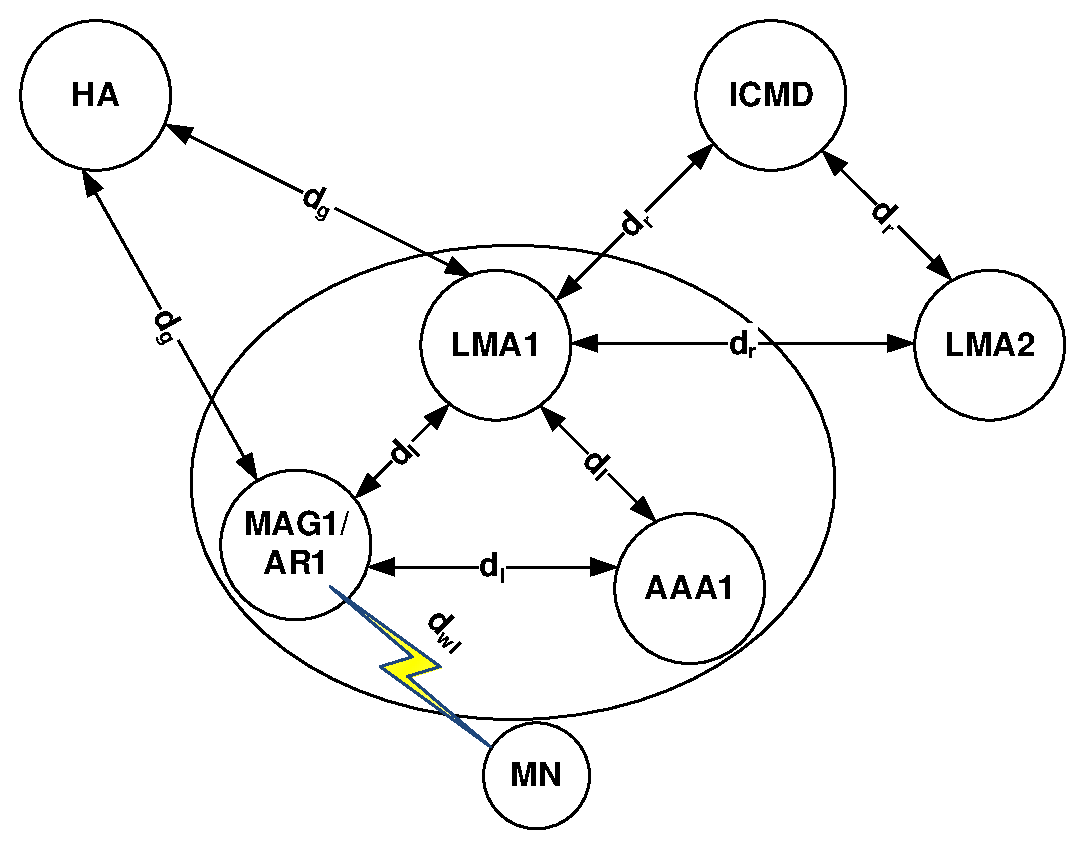
\includegraphics[width=0.55\textwidth]{./Part3/Chapter7/figures/c9_topology_analysis.eps}
\caption[Reference network topology for performance analysis.]{Reference network topology for performance analysis.}
\label{fig:c9_reference}
\end{figure}

Fig.~\ref{fig:c9_reference} shows a reference topology for performance analysis. For simplicity, the average distance (number of hops) between the entities is defined as follows:
\begin{itemize}
\item The distance between the PMIPv6 entities in the same domain (local) is d$_{l}$ (e.g., between the MAG and the LMA). 
\item The distance between two domains (region) is d$_{r}$ (e.g., between two LMAs or between the LMA and the ICMD).
\item The distance between LMA/AR and Home Agent (HA) (global) is d$_{g}$.  
\item The distance between the MAG/AR and the MN (wireless connection) is d$_{wl}$.
\end{itemize}

\subsection{Signaling Cost}
Signaling cost of a mobility management protocol is defined as the transmission cost of location update signaling when an MN performs handover. To measure the signaling cost in the inter-domain context, the handoff frequency should be taken into account. As a result, we use a well-known factor, called session-to-mobility ratio (SMR) which represents the relative ratio of session arrival rate to the user mobility rate.
It is assumed that the subnet residence time (MAG subnet) and session duration follows an exponential distribution with parameter $\eta$ and $\mu$, respectively. Hence, the SMR is calculated as $\rho=\frac{\mu}{\eta}$ \cite{prob}. 
Each LMA coverage area is supposed to be circular with N subnets. According to \cite{HO_comparison_Makaya}, the intra-domain and the inter-domain handoff probability are defined as $\rho_{intra}=\frac{1}{1+\rho}$,  $\rho_{inter}=\frac{1}{1+\rho \sqrt{N}}$. And the expected numbers of intra-handoff and inter-handoff are $E_{intra}=\dfrac{1}{\rho}$, $E_{inter}=\dfrac{1}{\rho \sqrt{N}}$
Thus, the average location update signaling is given by:\\
\begin{equation}
SC(.) = \left( E_{intra} - E_{inter}\right) SC_{intra} (.) + E_{inter} SC_{inter}(.),
\end{equation}
where $SC_{intra}$ and $SC_{inter}$ are signaling update cost for intra-domain and inter-domain handover, respectively. 
Although different signaling messages have different size, we assume that they have the same size for simplicity. Also, the cost for transmitting a signaling message is supposed to be proportional to the distance between source and destination. The proportion is $\alpha$ for wired and $\beta$ for wireless link. The signaling cost of DP-PMIP is calculated as: 
\setlength{\arraycolsep}{0.0em}
\begin{eqnarray}
SC_{intra} (DP-PMIP)&{}  ={}& 2 \beta d_{wl} + 2\alpha d_{l},\\
SC_{inter}(DP-PMIP)&{}  ={}&  2 \beta d_{wl} + 2\alpha d_{l} +4\alpha d_{r}. 
\end{eqnarray}

Similarly, we can derive the equations of the signaling cost for DF-PMIP, MIPv6 and H-PMIP. It is noted that the signaling cost for intra-domain handover of DF-PMIP and H-PMIP is the same and equal to that of DP-PMIP (PMIP handover cost). \\
\setlength{\arraycolsep}{1.0em}
\begin{eqnarray}
SC_{inter}(DF-PMIP)&{} ={}& 4\beta d_{wl} + 6\alpha d_{l} +4\alpha d_{r}. \\
SC_{inter}(MIP)&{} ={}& SC_{intra}(MIP) = 4 \beta d_{wl} + 2\alpha d_{g}. \\
SC_{inter}(H-PMIP)&{} ={}& 4\beta d_{wl} + 2\alpha d_{l} +2\alpha d_{g}.
\end{eqnarray}

\subsection{Handover Latency}
The Inter-domain handover latency ($HO_{inter}$) is defined as the total time taken to complete all the operations before the traffic can be forwarded to the current location of the MN. Let $HO_{intra}$ denote the intra-domain handover delay. Then, the average value of handover latency is
\begin{equation}
\label{DP-PMIP}
HO(.)  = \left( \rho_{intra} - \rho_{inter} \right) HO_{intra}(.) + \rho_{inter} HO_{inter}(.).
\end{equation}

Since the delay between two nodes depends on the bandwidth, the propagation delay and the distance between them, for simplicity, we suppose that the delay is proportional to the distance. The proportion is $ \tau$ for wired link and $\kappa$ for wireless link. 
Let t$_{L2}$ denote the delay caused by Layer 2 handover. Thus, the intra-domain handover delay of DP-PMIP, DF-PMIP and H-PMIP are the same (PMIP handover delay) and are calculated as follows:\\
\begin{equation}
\label{DP-PMIP-intra}
HO_{intra}(DP-PMIP) = t_{L2} + 2\kappa d_{wl} + 2\tau d_{l}. 
\end{equation}

On the other hand, the handover latency of DP-PMIP, DF-PMIP, MIPv6 and H-PMIP are given by the equations below.\\
\setlength{\arraycolsep}{0.0em}
\begin{eqnarray}
HO_{inter}(DP-PMIP)&{} ={}& t_{L2} + 2 \kappa d_{wl} + 2\tau d_{l} + 2\tau d_{r}. \\
HO_{inter}(DF-PMIP)&{} ={}& t_{L2} + 4 \kappa d_{wl} + 6\tau d_{l}+ 4\tau d_{r}. \\
HO_{inter}(MIP)&{} ={}& SD_{Intra}(MIP) = t_{L2} + 4\kappa d_{wl} + 2\tau d_{g}. \\
HO_{inter}(H-PMIP)&{} ={}& t_{L2} + 4\kappa d_{wl} + 2\tau d_{r} + 2\tau d_{g}. 
\end{eqnarray}
\subsection{Tunnel Usage}
In this subsection, we will measure the tunnel usage ratio, called $\theta$ which is calculated as the ratio between the number of sessions using the tunnel (between the anchor and the current domain) and the total number of sessions. Thus, it can be used to show the advantage of using DMM in terms of dynamic provision of mobility service. 

Since in MIPv6, H-PMIP and I-PMIP the traffic always passes the tunnel between the global anchor point and the current one, $\theta$ is equal to 1. 

To measure $\theta$ in case of D-PMIP, the sessions are separated into new sessions and handoff sessions. Thanks to DMM, the tunnel is used only for the handoff sessions. Let $N_{n}(t)$ and $N_{h}(t)$ denote the numbers of new sessions and handoff sessions up to time t, respectively. We suppose that $N_{n}(t)$ and $N_{h}(t)$ are a Poisson process with parameter $\lambda_{n}$ and $\lambda_{h}$, respectively. Thus, we have $\theta =\dfrac{N_{h}(t)}{N_{n}(t)+N_{h}(t)}$. According to \cite{prob} $\lambda_{h} = E[H] * \lambda_{n}$, where E[H] is the handoff rate (in our case E[H] = $\frac{1}{\rho\sqrt{N}}$). 
Thus, we obtain:
\begin{equation}
\theta = \dfrac{1}{ 1+ \rho\sqrt{N}}.       
\end{equation}

\subsection{Multicast Service Disruption Time}
Similar to the handover latency, the multicast service disruption time ($SD(.)$) is defined as\\
 \begin{equation}
SD(DP-PMIP)= \left( \rho_{intra} - \rho_{inter} \right) SD_{intra}(DP-PMIP) + \rho_{inter} SD_{inter}(DP-PMIP),
\end{equation}
where $SD_{intra}(DP-PMIP)$ and $SD_{inter}(DP-PMIP)$ are the multicast service disruption time for intra- and inter-domain mobility, respectively. As can be seen in Fig.~\ref{fig:c9_multicast_signaling}, $SD_{inter}(DP-PMIP)$ is calculated as\\
\begin{equation}
SD_{inter}(DP-PMIP) = t_{L2} + 2\kappa d_{wl} + 4\tau d_{l} + 4\tau d_{r} + 2 max \{ \tau d_{l}, \tau d_{r} \}. 
\end{equation}
The multicast service disruption, in case of intra-domain handover is given by (see Chapter \ref {ch:multicast_PMIP})
\begin{equation}
SD_{intra}(DP-PMIP) = t_{L2} + 2 \kappa d_{wl} + 6\tau d_{l}. 
\end{equation}

On the other hand, the average multicast service disruption time in PMIPv6 is given by\\
\begin{equation}
SD(PMIP) = \rho_{intra} SD_{intra}(DP-PMIP). 
\end{equation}

\section{Numerical Results} \label{ch9:numerical_result}
This section presents the numerical results based on the analysis given in the previous section. The default parameter values for the analysis are introduced in Table ~\ref{tap:c9_parameters} in which some parameters are taken from \cite{HO_comparison_Makaya}. \\

\begin{table}[ht]
\caption[Inter-mobility domain solution: Parameters for the performance analysis]{Parameters for Performance Analysis}
\label{tap:c9_parameters}
\centering
\begin{tabular}{|c |c |c |c |}
\hline
Parameters & Values & Parameters & Values\\
\hline
d$_{wl}$ & 1 hops &d$_{l}$ & 6 hops \\
\hline
 d$_{r}$ & 6 hops & d$_{g}$ & 12 hops \\
 \hline
$\tau$ & 2 & $\kappa$ & 15  \\
\hline
N & 32 & $\alpha$ & 1 \\
\hline
$\beta$ & 5  & $t_{L2}$ & 50ms \\
\hline

\end{tabular}
\end{table}

\begin{figure}[h!]
\centering
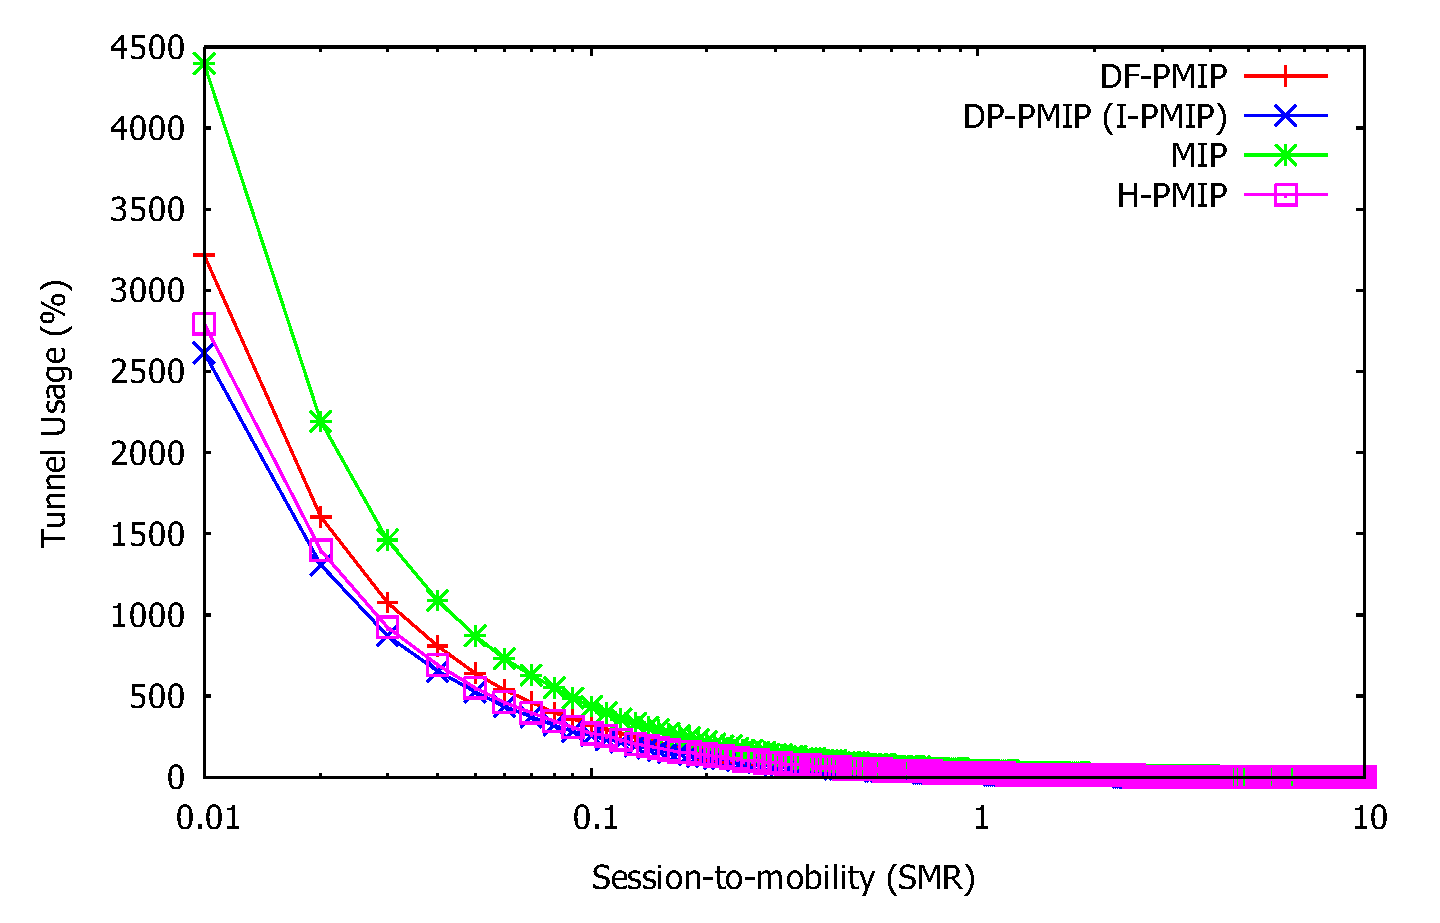
\includegraphics[width=0.50\textwidth]{./Part3/Chapter7/figures/c9_signaling_cost_smr_6.eps}
\caption[Signaling cost as a function of the session-to-mobility.]{Signaling cost variation with SMR ($\rho$).}
\label{fig:signaling_cost}
\end{figure}

Fig.~\ref{fig:signaling_cost} shows the signaling cost when SMR ($\rho$) is varying. We can observe that the signaling cost of the fully distributed solution is relatively high compared to the other. It is evident since more messages are required to get the address of the anchor LMA. The partially distributed solution and I-PMIP have lower signaling cost than that of the others. In highly mobile regimes ($\rho\ll1$), the difference between the protocols becomes more clearly. 

Fig.~\ref{fig:Handover_latency} illustrates the handover latency as a function of SMR. The partially distributed solution (DP-PMIP) has better handover latency (lower is better) over the other solutions especially when $\rho$ is small (in highly mobile regimes). 
\begin{figure}
\centering
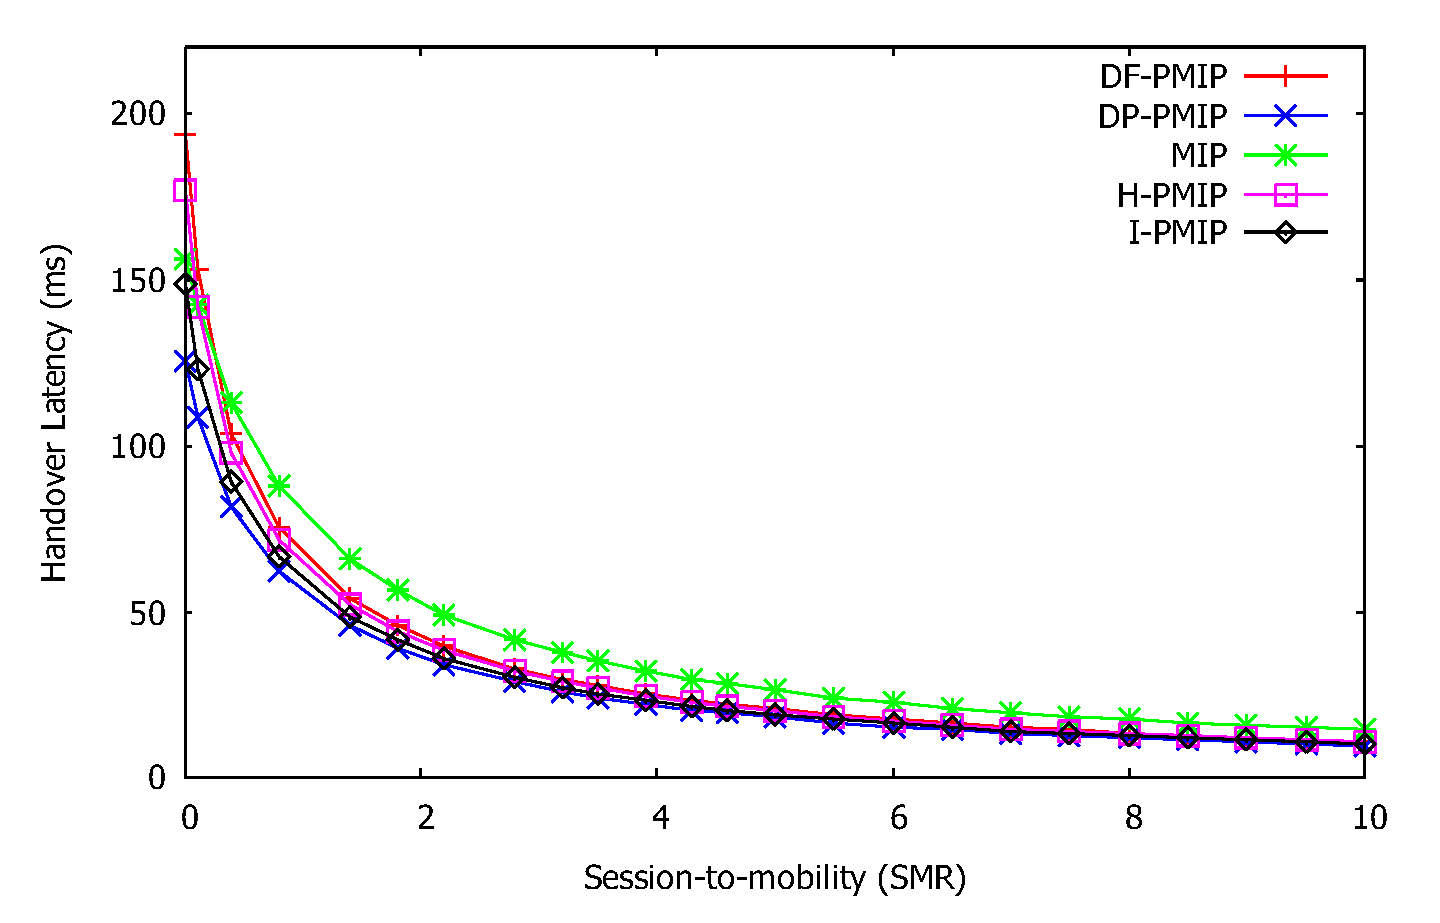
\includegraphics[width=0.50\textwidth]{./Part3/Chapter7/figures/c9_handover_smr_6.eps}
\caption[Handover latency as a function of the session-to-mobility.]{Handover latency variation with SMR ($\rho$).}
\label{fig:Handover_latency}
\end{figure}

To measure the impact of domain size on the handover latency, we assume that the architecture of the inter-domain is hierarchically formed as a tree structure with a $d_{r}$-layer, while the structure of a PMIPv6 domain as a binary tree with a $d_{l}$-layer \cite{multicast_mobileIP}. The size of the network is supposed to be fixed e.g., the distance between the ICMD and MAG is 12 hops. Therefore, $d_{l}$ and $d_{r}$ are calculated as $d_{l}=log_{2}(N)$, $d_{r} = 12 - log_{2}(N)$. Fig.~\ref{fig:domain_size} describes the impact of domain size on handover latency when the value of $\rho$ is set to 0.1. It is observed that when the domain size is small, the handover latency is high for all solutions. When the domain size is increased, the handover latency is decreased and then makes a bit increase. 
\begin{figure}[h!]
\centering
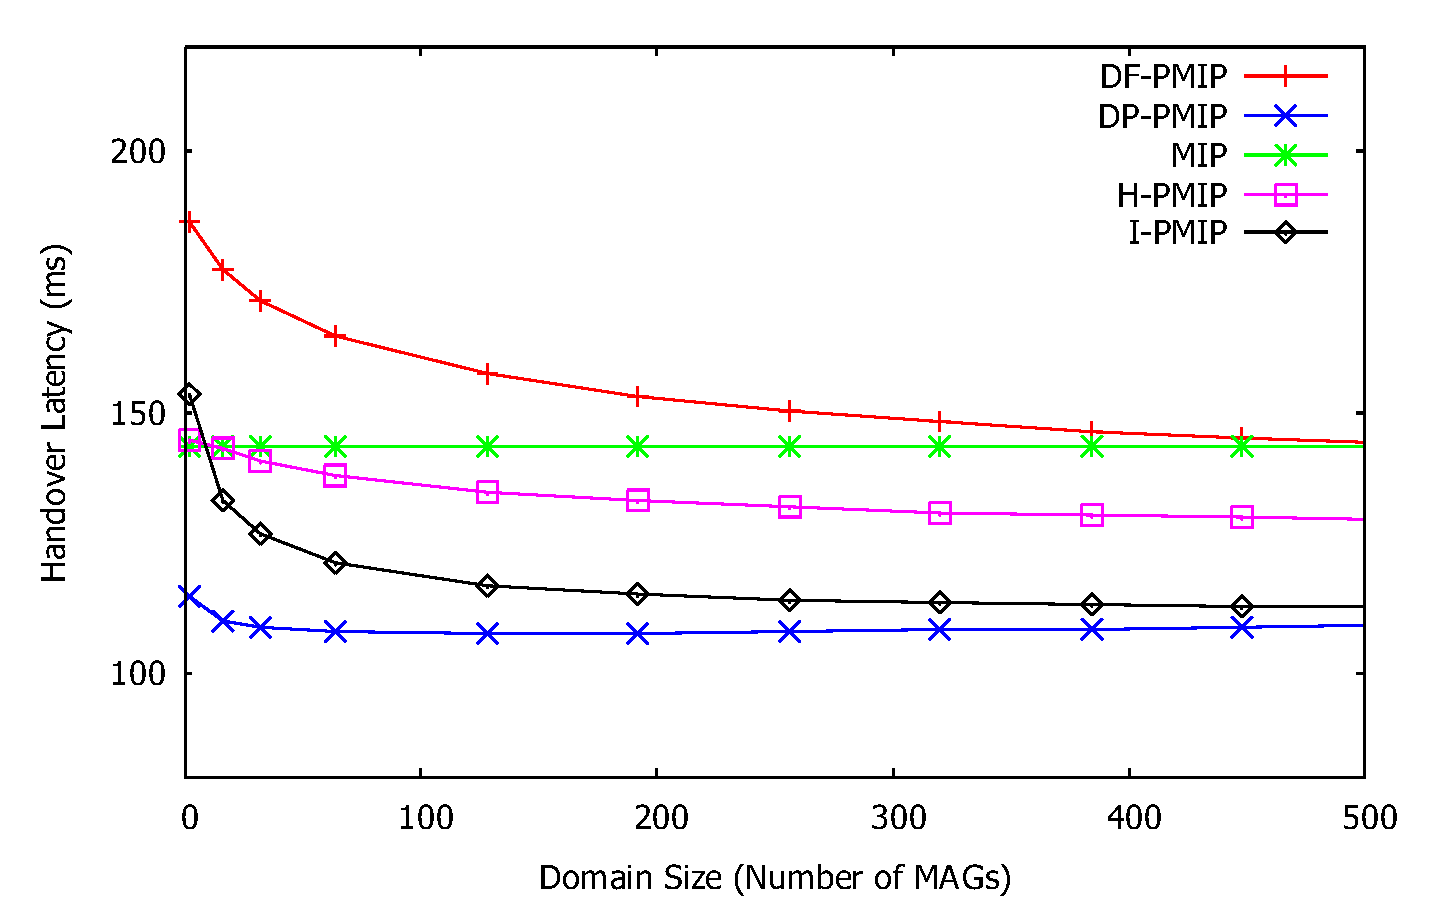
\includegraphics[width=0.50\textwidth]{./Part3/Chapter7/figures/c9_domain_size_6.eps}
\setlength{\belowcaptionskip}{-10pt}
\caption[The impact of domain size on the handover latency.]{Domain size effect.}
\label{fig:domain_size}
\end{figure}

The tunnel usage as a function of SMR is illustrated in Fig.~\ref{fig:tunnel_usage}. In low mobility regimes ($\rho\gg1$) the tunnel usage is significantly decreased in D-PMIP (DP-PMIP, DF-PMIP) compared to the others. The reason is that the number of new sessions in low mobility regimes is definitely higher than that of handoff sessions.
\begin{figure}[h!]
\centering
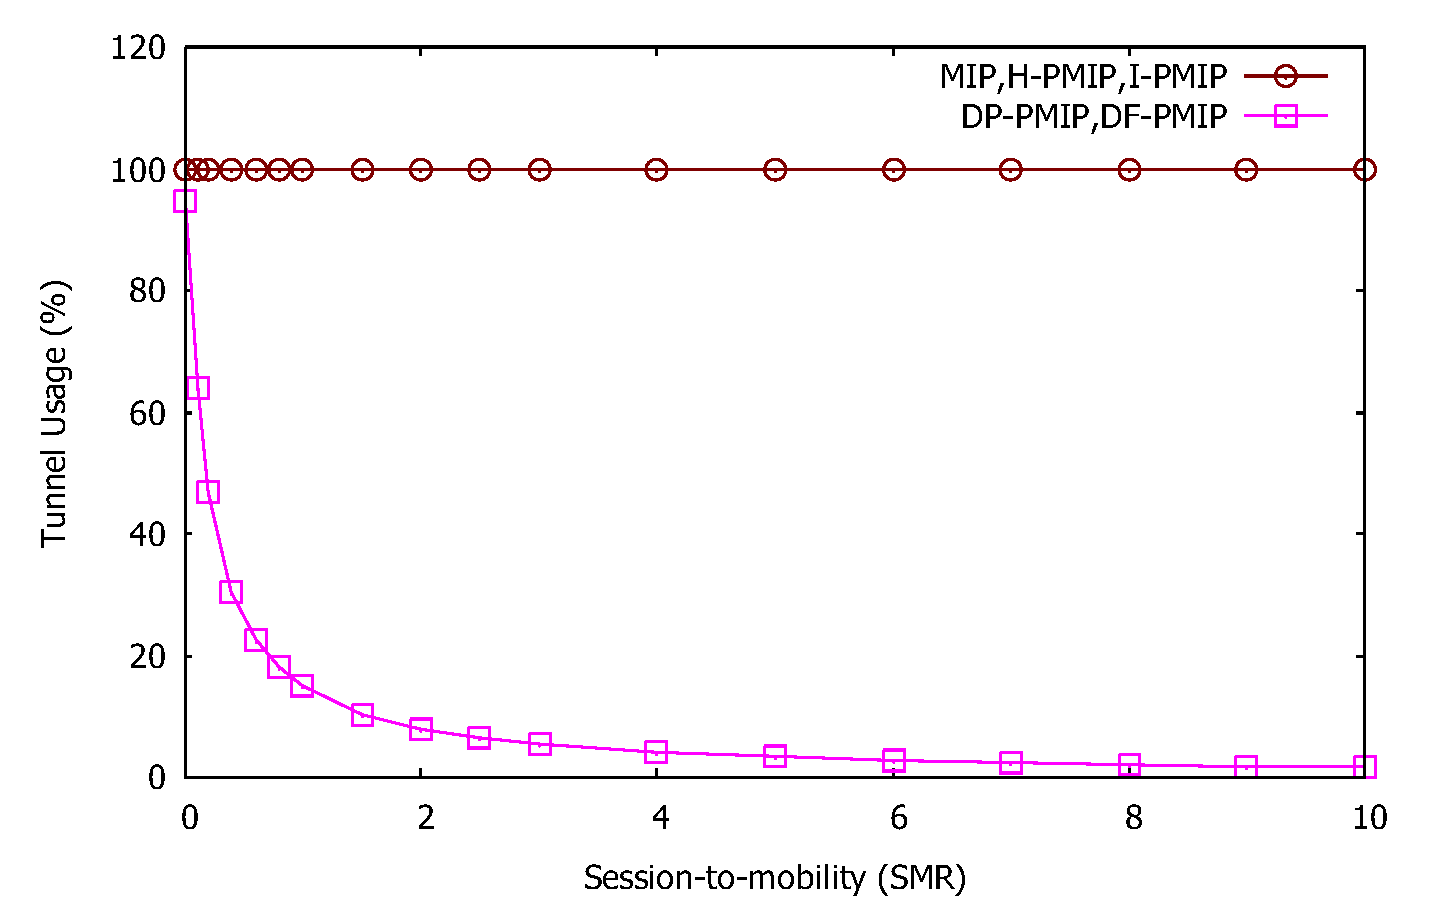
\includegraphics[width=0.50\textwidth]{./Part3/Chapter7/figures/c9_tunnel_usage.eps}
\caption[Tunnel usage.]{Tunnel usage ($\theta$) as a function of SMR ($\rho$).}
\label{fig:tunnel_usage}
\end{figure}

Finally, Fig.~\ref{fig:multicast} plots the average multicast service disruption time as a function of SMR. We can observe that the average service disruption in case of DP-PMIP is slightly greater than that in case of intra-handover inside PMIPv6. It is because inter-domain handover latency is typically greater than that in case of intra-domain handover. 

\begin{figure}[h!]
\centering
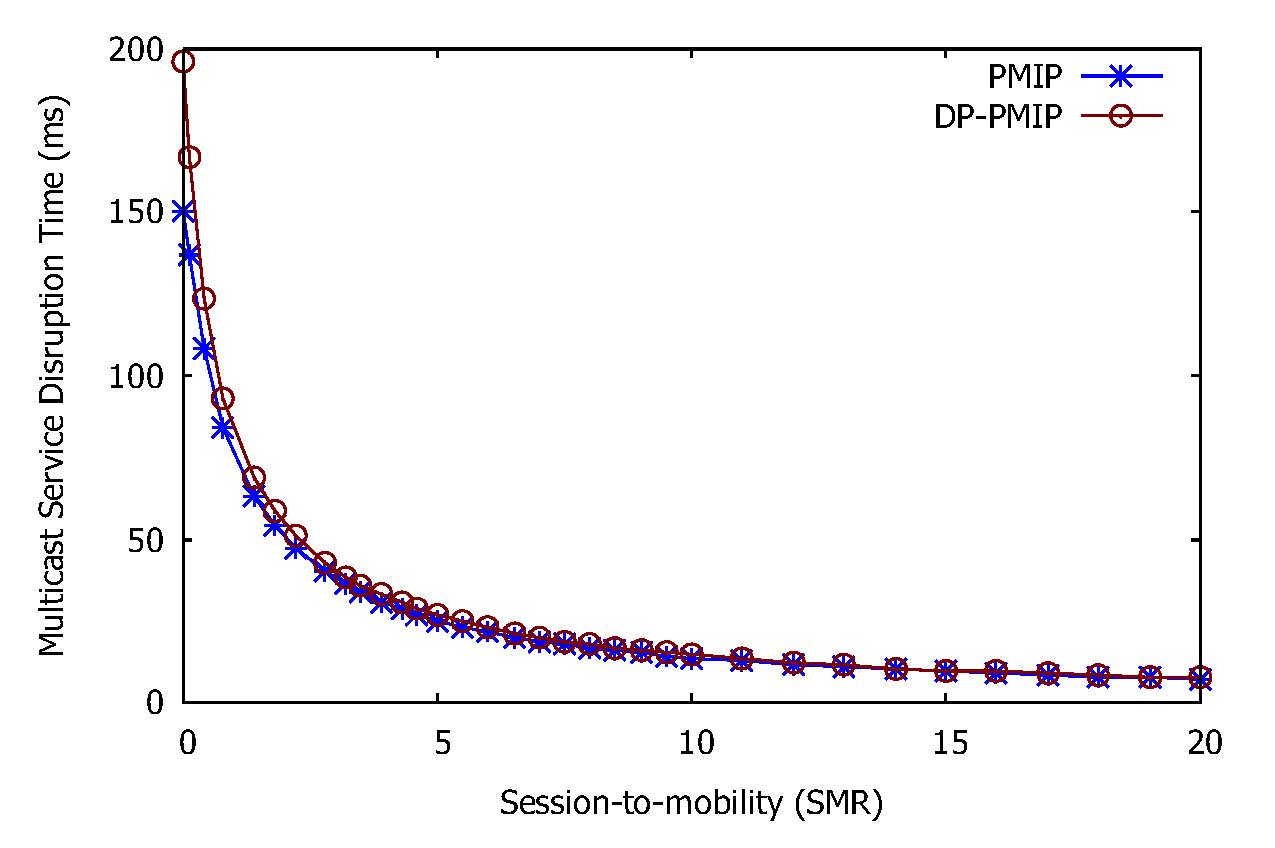
\includegraphics[width=0.50\textwidth]{./Part3/Chapter7/figures/c9_multicast.eps}
\caption[Multicast service disruption time as a function of the session-to-mobility.]{Multicast service disruption time as a function of SMR ($\rho$).}
\label{fig:multicast}
\end{figure}

\section{Conclusion} \label{ch9:conclusion}
This chapter proposes a solution (D-PMIP) that allows providing mobility service for the moving hosts between PMIPv6 domains. Based on the DMM concept, the proposal allows bringing the mobility anchors closer to the MN and dynamically providing the mobility service for only sessions which really need the service continuity. The D-PMIP also retains the advantageous features of a network-based mobility management form PMIPv6 that provides mobility service without the involvement of the MN. A numerical analysis demonstrates that the partially distributed solution gives better performance than the other solutions like MIPv6, H-PMIP, I-PMIP and the fully distributed solution in terms of signaling cost, handover latency and tunnel usage. Thus, at the moment the partially distributed solution seems to be more suitable than the fully distributed one. 

The proposed solutions can be considered as a DMM-like approach applying to the existing PMIPv6 network to improve the mobility of the nodes. We then present a basic support for the multicast mobility in the partially distributed scheme. It allows keeping the MN unaware of mobility from the multicast service perspective. Also, the multicast service disruption time is slightly increased compared to the mobility inside a single PMIPv6 domain. 
